
\section{Example: Validating PISM as a flow model for the Ross ice shelf (EISMINT-Ross)}\label{sect:ross} \index{PISM!running the EISMINT-Ross ice shelf intercomparison in}\index{Ice Sheets!Antarctic ice sheet!Ross ice shelf} \index{EISMINT!intercomparison of Ross ice shelf models} \index{PISM!validation of ice shelf model} \index{Ross ice shelf}
\optsection{EISMINT-Ross}

The term ``validation'' describes the comparison of model output with physical observations in cases where those physical observations are believed to be sufficiently complete and of sufficient quality so that the performance of the numerical model can be assessed \cite{Roache,Wesseling}.  Roughly speaking, validation can happen when the observations or data are better than the model, so the comparison measures the quality of the numerical model and not merely errors in, incompleteness of, or lack of confidence in, the data.

As part of the first EISMINT series of intercomparisons, MacAyeal and others \cite{MacAyealetal} validated several ice shelf numerical models using the Ross ice shelf as an example.  We refer to this intercomparison and its associate write-up \cite{MacAyealetal} as ``EISMINT-Ross''.  The models were compared to data from RIGGS (the Ross Ice shelf Geophysical and Glaciological Survey \cite{RIGGS2,RIGGS1}), acquired in the period 1973--1978.   The RIGGS data include the (horizontal) velocity of the ice shelf measured at a few hundred locations in a reasonably regular grid across the shelf; see figure \ref{fig:rosspython} below for an indication of these positions.

Substantial developments have occurred in the modeling of the Ross ice shelf since the EISMINT-Ross intercomparison.  For example, inverse modeling techniques were used to recover depth-averaged viscosity of the Ross ice shelf from the RIGGS data in \cite{RommelaereMacAyeal}. A parameter-sensitivity study was performed for a particular Ross ice shelf numerical model in \cite{HumbertGreveHutter}.

The scripts in this section are found in the directory \texttt{examples/eisross/}.  The script \texttt{quickstart.sh} in that directory will download the data, build a NetCDF input file, and run \texttt{pross} as described in the next three subsections.

\subsubsection*{Grabbing the data}  Download data files from the website:

\centerline{\url{http://homepages.vub.ac.be/~phuybrec/eismint/iceshelf.html}}
\small

\begin{verbatim}
$ cd examples/eisross/
$ wget http://homepages.vub.ac.be/~phuybrec/eismint/111by147Grid.dat
$ wget http://homepages.vub.ac.be/~phuybrec/eismint/kbc.dat
$ wget http://homepages.vub.ac.be/~phuybrec/eismint/inlets.dat
\end{verbatim}
\normalsize The reader might want to look at these files in a text editor.  Their idiosyncratic format must be handled by a python script, namely \texttt{eisross.py} below.  In fact, a significant part of setting up EISMINT-Ross in PISM was the step of converting these text files into a machine-readable and metadata-containing NetCDF file.  The next script\footnote{Requires \href{http://numpy.scipy.org/}{\texttt{numpy}} and \href{http://code.google.com/p/netcdf4-python/}{\texttt{netcdf4-python}}.} reads the above three \texttt{.dat} files and it creates a NetCDF file:

\begin{verbatim}
$ ./eisross.py -o ross.nc
\end{verbatim}
Note that the NetCDF file \texttt{ross.nc} can be reconverted to text (CDL) using \texttt{ncdump} or it can be viewed graphically with \texttt{ncview}.  For example, \texttt{ncdump -h ross.nc} shows the ``header'' (the metadata) for \texttt{ross.nc}.  The script \texttt{eisross.py} has added this metadata, much of which can only be found by carefully reading references \cite{RIGGS2,RIGGS1,MacAyealetal}.

\begin{figure}[ht]
\centering
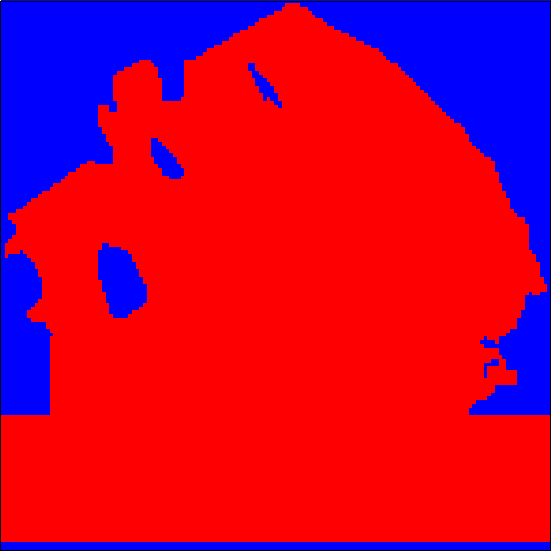
\includegraphics[height=2.3in,keepaspectratio=true]{rossmask} \qquad 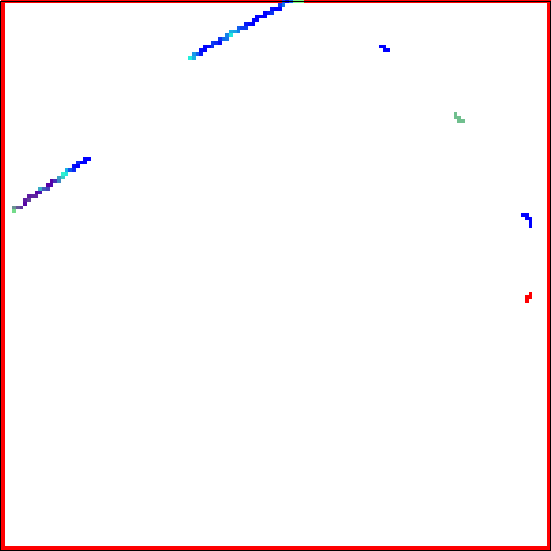
\includegraphics[height=2.3in,keepaspectratio=true]{rossubar}
\caption{Two views from \protect{\texttt{ncview}} of the EISMINT-Ross data in the NetCDF file \protect{\texttt{ross.nc}}.  The floating-versus-grounded mask (left; red areas are floating ice shelf) and the $x$-component of the non-zero kinematic (Dirichlet) boundary condition for velocity (right).}
\label{fig:rossmaskubar}
\end{figure}

The NetCDF file \texttt{ross.nc} contains ice thickness, bed elevations, surface temperature, and accumulation.  Values for latitude and longitude from the RIGGS survey grid \cite{RIGGS1} are given.  All of these are typical of ice sheet modeling data, both in evolution and diagnostic runs.  The file also has variables \texttt{ubar} and \texttt{vbar}.  These give the boundary values which are needed for the diagnostic computation of velocity, and they are only valid at grounding line locations.  They are the measured velocities of the ice flow inputs to the ice shelf.  Also present are integer variables \texttt{mask}, which shows the domain where the ice shelf is modeled and the locations where the boundary conditions are to be applied.  Finally, \texttt{ross.nc} contains variables which allow us to partly validate our computation.  There is an interger variable \texttt{accur} which flags the region where the interpolated measured velocities are believed to be accurate enough for validation.\footnote{\texttt{111by147.dat} has a ``Reliable Velocity Obs'' flag.}  The variables \texttt{azi_obs} and \texttt{mag_obs} are believed to be accurate in this region \cite{MacAyealetal}.

The original EISMINT-Ross data are on a 111 by 147 grid but \texttt{eisross.py} extends this grid to a more convenient 147 by 147 grid with the same $6.822$ km spacing.  This grid has ice-free ocean beyond the calving front, which is straightened as described in \cite{MacAyealetal}.  The gridded data have a particular resolution, but the PISM computational grid can be finer or coarser according to runtime options (as illustrated below).

\subsubsection*{Diagnostic computation of ice shelf velocity}  A basic Ross ice shelf velocity computation from these data is:

\begin{verbatim}
$ pross -boot_file ross.nc -Mx 147 -My 147
\end{verbatim}%$
Here we initialize from \texttt{ross.nc}. The computational grid specified here is the $6.822$ km data grid in EISMINT-Ross with 147 grid points in each direction.  The maximum thickness of the ice is $874$ m so we choose a height for the computational box (\texttt{-Lz}) large enough to contain the ice.  Note that using a small number of vertical levels (\texttt{-Mz 3}) is reasonable because the EISMINT-Ross intercomparison specifies that the temperature at each depth is just the surface temperature \cite{MacAyealetal}.  In fact there is no thermocoupling issue because the ice hardness used here is constant.

The executable \texttt{pross} was created especially for this modeling example. It demonstrates PISM's ability to diagnostically model the Ross ice-sheet \emph{and} serves as an example of using PISM components as software libraries. PISM does not have generic mechanisms for diagnostic modeling of the flow in ice shelves or for specifying in-flow boundary conditions such as used in this case. This kind of work will require extending PISM by writing additional code, and looking at \texttt{pross.cc} is a reasonable place to start.

This particular case of diagnostic modeling does not require solving either temperature\footnote{Recall that the ice hardness is set to a constant.} or mass-continuity equations, so \texttt{pross} only uses the part of PISM responsible for shallow stress balance computations. This means that ``bootstrapping'' in this section differs from bootstrapping in section \ref{sect:boot}. You do have to specify \texttt{Mx} and \texttt{My}, but other parameters are determined from the input file and no heuristics are used to make up for missing data.

At the end of this run the computed velocity field is compared to the interpolated observed velocities stored in \texttt{ross.nc}.  The value called ``average relative error in vector vel'' is most relevant.  A value of 0.07 here means that the averaged absolute difference between the computed and the observed velocity, in the ``accurate'' region, is 7\%.

The output file \texttt{unnamed_diag.nc} contains vertically-averaged horizontal speed in the variable \texttt{cbar}.  Figure \ref{fig:rosspython} shows that computed speed as the color background; the comparison of modeled and observed vector velocities in that figure is discussed below.

There are many variations on this basic ``\texttt{pross}'' run above.  First of all one can get more information during the run by adding diagnostic viewers and a more complete (verbose) report to standard out:
\begin{verbatim}
$ pross -boot_file ross.nc -Mx 147 -My 147 \
        -view_map cbar,mask,velbar -verbose -pause 10
        -ssa_view_nuh
\end{verbatim}
Secondly one might want to do the run in parallel and do it on a finer grid.  For example,

\begin{verbatim}
$ mpiexec -n 4 pross -boot_file ross.nc \
          -Mx 201 -My 201
\end{verbatim}
The result is very similar, as it should be.  On the other hand, since the data is only on a 6.8 km grid we expect no added accuracy on this new 5km grid.

Alternately one might want to experiment with different values of the hardness parameter.  Its default value is $\bar B = 1.9 \times 10^8 \, \text{Pa}\, \text{s}^{1/3}$ as in \cite{MacAyealetal}.   We can also use smaller (more severe) tolerances for the nonlinear iteration (\intextoption{ssa_rtol}) and the linear iteration (\intextoption{ksp_rtol}) to get more confidence in the numerical scheme:

\begin{verbatim}
$ pross -boot_file ross.nc -Mx 147 -My 147 \
        -ice_custom_hardness 1.8e8 \
        -o ross_out_1p8.nc -ssa_rtol 1e-6 -ksp_rtol 1e-10
\end{verbatim}


\subsubsection*{Comparison to RIGGS data}  The file \texttt{riggs_clean.dat} is a cleaned-up version of the original RIGGS\index{RIGGS} data \cite{RIGGS1, RIGGS2}.  (See \texttt{README} for more explanation on this RIGGS data.)  To convert this data to a NetCDF file, as needed next, do

\begin{verbatim}
./riggs.py -o riggs.nc
\end{verbatim}
A file \texttt{riggs.nc} will be created.  This data is one-dimensional; it is just a lists of values which have an index dimension \texttt{count} in the NetCDF file \texttt{riggs.nc}.

Now, \texttt{pross} can read this data and compute a $\chi^2$ statistic comparing computed PISM output to the data:

\small
\begin{verbatim}
$ mpiexec -n 2 pross -boot_file ross.nc -Mx 147 -My 147 \
          -riggs riggs.nc -o rossComputed.nc
PROSS trunk 0.3.1449 (EISMINT-Ross diagnostic velocity computation mode)
. . .
* Initializing the SSA stress balance...
  [using the finite difference implementation]
* Solving the SSA stress balance ...
comparing to RIGGS data in riggs.nc ...
. . .
Chi^2 statistic for computed results compared to RIGGS is   3680.748
maximum computed speed in ice shelf is   1401.166 (m/a)
ERRORS relative to observations of Ross Ice Shelf:
. . .
 average relative error in vector vel =   0.07168
\end{verbatim}
\normalsize

Naturally, the question is ``does this $\chi^2$ value of $3681$ represent a good fit of model result to observations''?  Also naturally, there is no objective answer.  For comparison, Table 1 in \cite{MacAyealetal} is reproduced here as Table \ref{tab:chisqr}.  As noted, all these results are with a constant hardness parameter $\bar B = 1.9 \times 10^8 \, \text{Pa}\, \text{s}^{1/3}$ \cite{MacAyealetal}. The maximum computed horizontal ice speed above of $1401$ m/a is slightly lower than the maximum velocities reported by some other models but, on the other hand, the maximum measured speed in the RIGGS data set is $1007$ m/a (occurring near the calving front, naturally).  The $\chi^2$ result is essentially as good as the best in the Table, noting smaller $\chi^2$ is better.

\small
\begin{table}[ht]
\centering
\caption{Model performance index, $\chi^2$ (non-dimensional).  \protect{\textsl{(Reproduction of Table 1 in \cite{MacAyealetal}.)}}}\label{tab:chisqr}
\begin{tabular}{p{0.2\linewidth}p{0.1\linewidth}p{0.3\linewidth}}\toprule
\textsl{Model} & $\chi^2$ & \textsl{Maximum velocity, m/year} \\\midrule
Bremerhaven1 & 3605 & 1379 \\
Bremerhaven2 & 12\,518 & 1663 \\
Chicago1 & 5114 & 1497 \\
Chicago2 & 5125 & 1497 \\
Grenoble & 5237 & 1508 \\
\bottomrule
\end{tabular}
\end{table}
\normalsize

\subsubsection*{Tuning the ice hardness for a better fit to RIGGS}  Because there is a relatively rich data set from RIGGS on ice velocity, it is reasonable to ask whether the PISM computed velocities can fit the data better if the spatially-constant hardness parameter $\bar B$ is adjusted.  In directory \texttt{examples/eisross/} there is a Python script \texttt{tune.py} which (by default) runs \texttt{pross} with seven values of $\bar B$ ranging from $\bar B = 1.6  \times 10^8$ to $\bar B = 2.2 \times 10^8 \, \text{Pa}\, \text{s}^{1/3}$.  It uses smaller values for the convergence tolerances (by default), yielding slightly different $\chi^2$ values.  It can be run in parallel: ``\texttt{\$ ./tune.py -n 4}.''

One sees that hardnesses $\bar B = 1.9,2.0 \times 10^8 \, \text{Pa}\, \text{s}^{1/3}$ give the best fits, by the standard of $\chi^2$ relative to RIGGS data.  This fitting exercise is a first small step towards inverse modelling of the spatially-distributed effective viscosity.  Another major tunable parameter, not demonstrated with \texttt{tune.py}, is the calving front force boundary condition.  More steps in the inverse modeling direction, for modeled velocity in Antarctic ice shelves, are found in \cite{HumbertGreveHutter,RommelaereMacAyeal}.


\subsubsection*{Additional visualization}  The visualization abilities of PISM's runtime viewers, and of \texttt{ncview} for NetCDF files, are limited.  On the other hand, we can produce pretty pictures using Python.  The script \texttt{rossplot.py} uses Python packages \texttt{netcdf4-python}, \texttt{matplotlib}, and \texttt{scikits.delaunay} to do this.  Assuming that files \texttt{ross.nc} and \texttt{rossComputed.nc} were produced as described previously, and are in the current directory, and that file \texttt{riggs_clean.dat} is present in the current directory too, then we can do:

\begin{verbatim}
$ ./rossplot.py
\end{verbatim}

\noindent We get Figure \ref{fig:rosspython}.  We have succeeded in modeling the flow in a real ice shelf.

\begin{figure}[ht]
\centering
\mbox{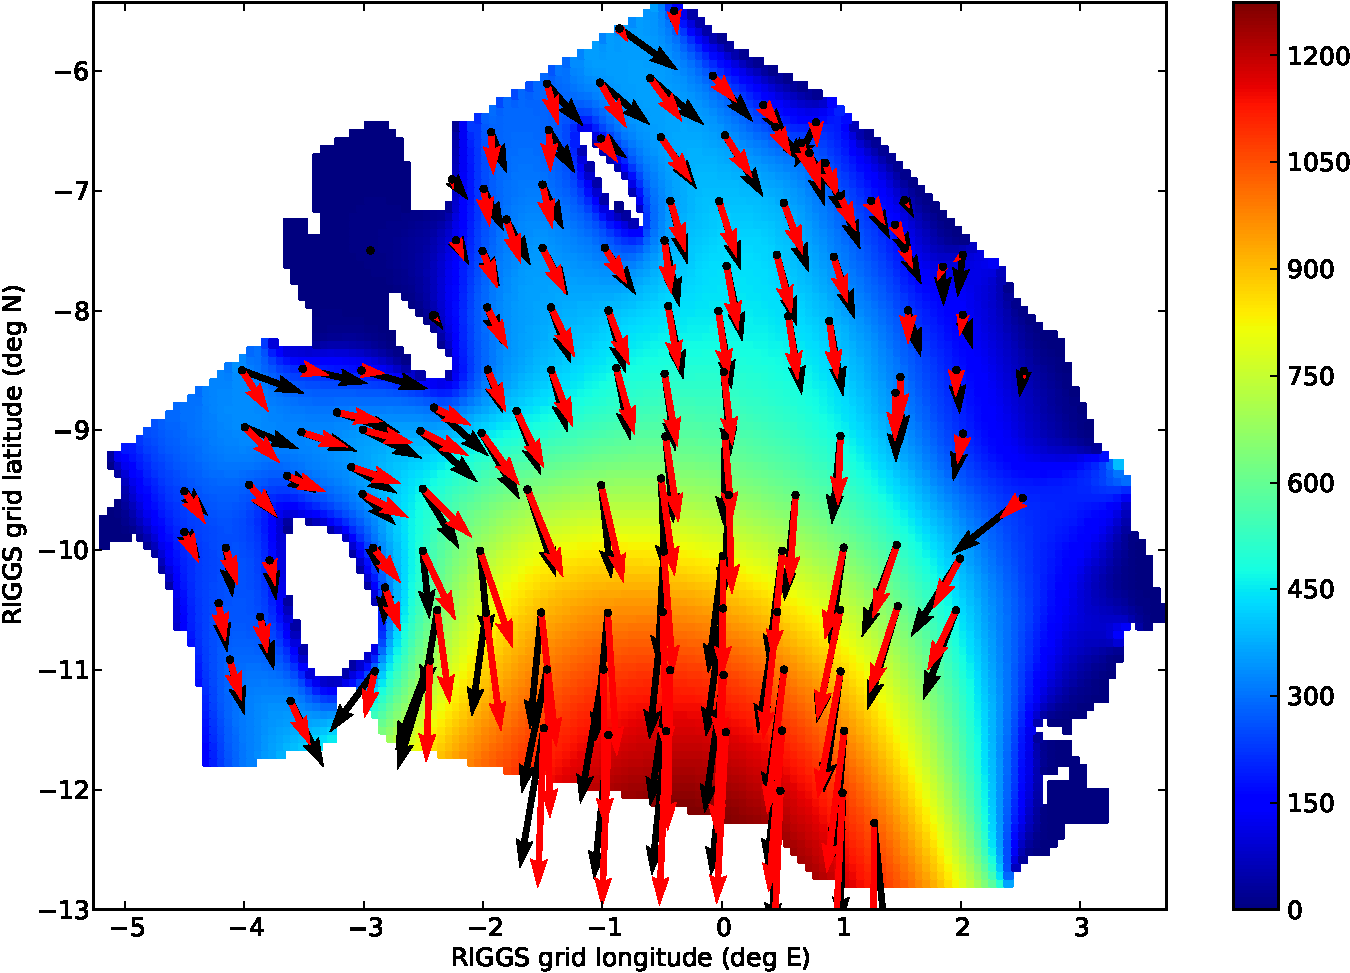
\includegraphics[width=3.3in,keepaspectratio=true]{rossquiver}\quad 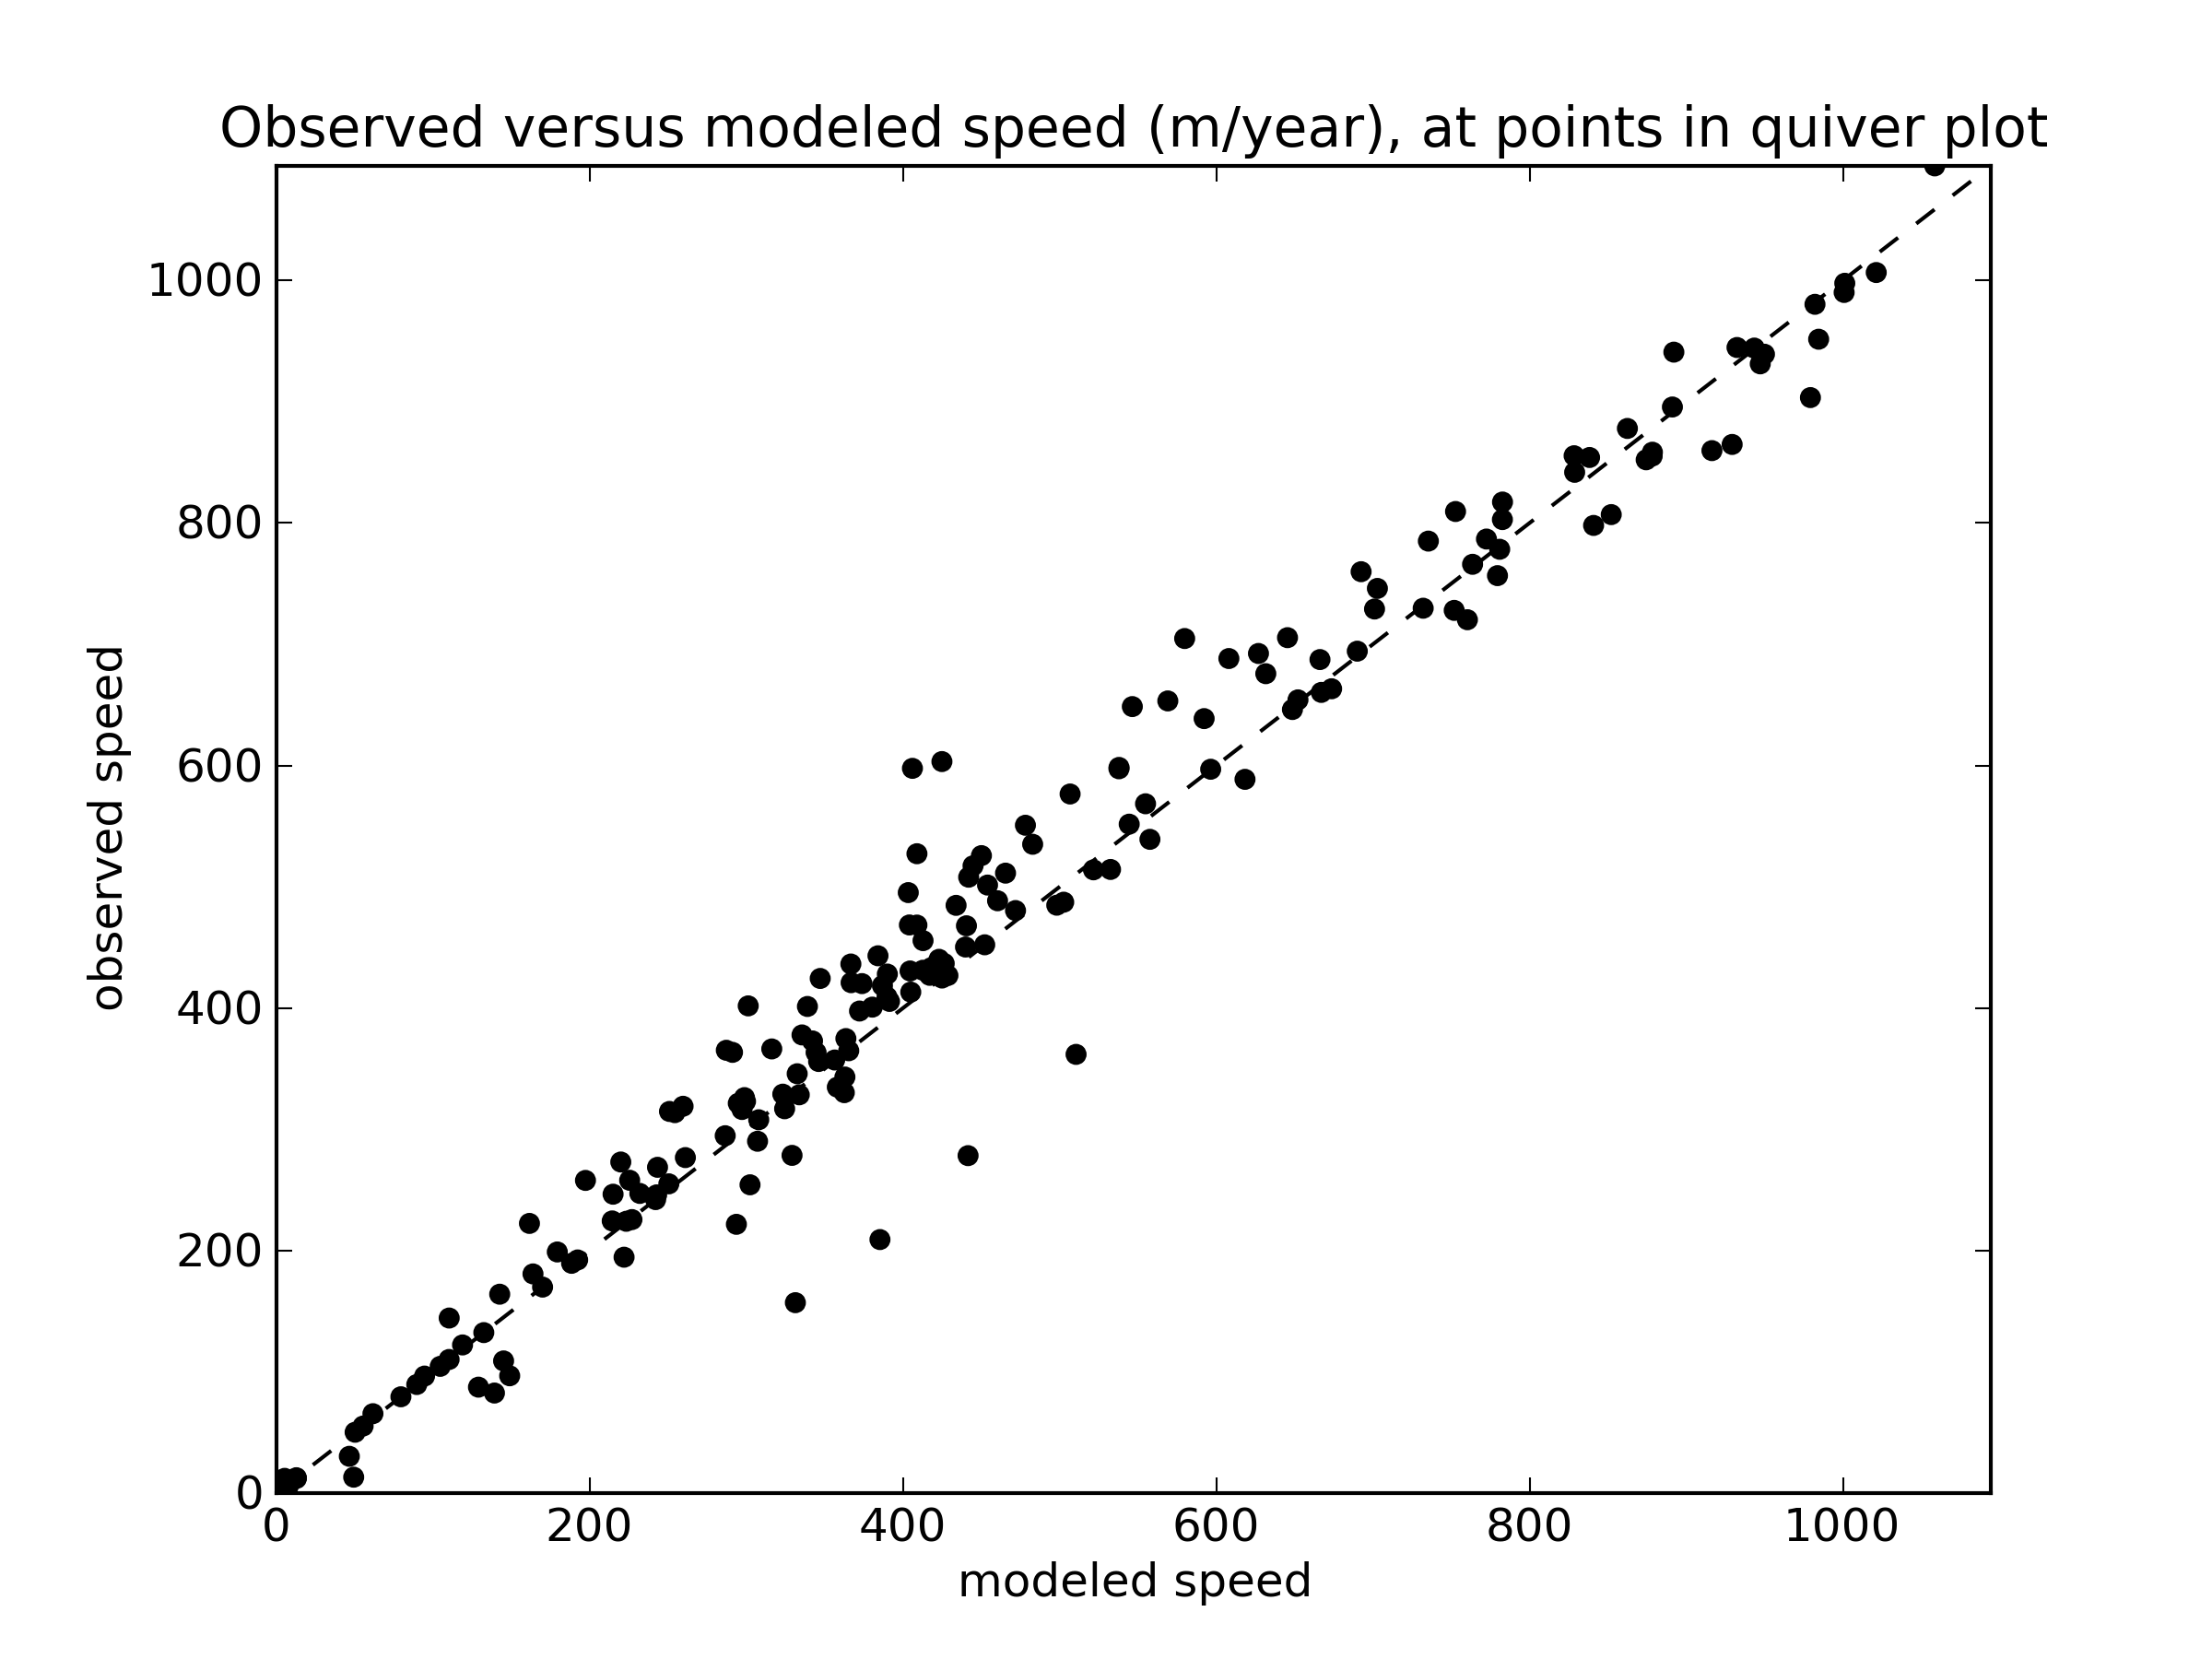
\includegraphics[width=2.7in,keepaspectratio=true]{rossscatter}}
\caption{\protect{\emph{Left}}: Color is speed in m/a.  Arrows are observed (black) and computed (red) velocities at RIGGS points.  \protect{\emph{Right}}: Comparison between modeled and observed speeds at RIGGS points; compare Figure 2 in \cite{MacAyealetal}.}
\label{fig:rosspython}
\end{figure}


%%% Local Variables: 
%%% mode: latex
%%% TeX-master: "manual"
%%% End: 
